\documentclass[a4paper]{book}

%%% INICIO DEL PREÁMBULO %%%

\usepackage[utf8]{inputenc}
\usepackage[greek,spanish,es-tabla,es-nodecimaldot,es-noindentfirst]{babel}
\usepackage{babelbib}
\usepackage{nccmath}
\usepackage{amsthm}
\usepackage{lipsum}
\usepackage{tcolorbox}
\usepackage[thicklines]{cancel}
\usepackage{mathtools}
\usepackage{amssymb}
\usepackage{amsmath}
\usepackage{caption}
\usepackage{subcaption}
\usepackage{color}
\usepackage{verbatim}
\usepackage{enumerate}
\usepackage{geometry}
\geometry{a4paper,left=35mm,right=35mm,top=15mm,bottom=15mm}
\usepackage{isotope}
\usepackage{maybemath}
\usepackage{upgreek}
\usepackage{wasysym}
\usepackage[italic]{hepparticles}
\usepackage{subdepth}
\usepackage{siunitx}
\sisetup{
	mode 			= text,
	parse-units 	= false
}
\usepackage{physics}
\usepackage{braket}
\usepackage{tensor}
\usepackage{chemformula}
\usepackage{tikz}
\usepackage{url}
\usepackage{listings}
\usepackage{multirow}
\usepackage{multicol}
\usepackage[colorlinks=true]{hyperref}
\hypersetup{
	citecolor = blue,
	linkcolor = blue,
	urlcolor = blue,
	pdfauthor = {Javier Rodrigo López}
}
\usepackage{eso-pic}

% tikz
\usepackage{tikz} \usetikzlibrary{fit,babel,shapes,arrows,patterns,positioning,calc,decorations.pathmorphing,decorations.markings}
\tikzstyle{block} = [draw, fill=white, rectangle,
minimum height=3em, minimum width=6em]
\tikzstyle{sum} = [draw, fill=white, circle, node distance=1cm]
\tikzstyle{input} = [coordinate]
\tikzstyle{output} = [coordinate]
\tikzstyle{pinstyle} = [pin edge={to-,thin,black}]
\tikzset{
	block/.style = {draw, fill=white, rectangle, minimum height=3em, minimum width=3em},
	tmp/.style  = {coordinate},
	sum/.style= {draw, fill=white, circle, node distance=1cm},
	input/.style = {coordinate},
	output/.style= {coordinate},
	pinstyle/.style = {pin edge={to-,thin,black}}
}

\usepackage[oldvoltagedirection]{circuitikz}
\usepackage{pdflscape}

% Títulos
\usepackage{titlesec}
\titleformat{\section}{\normalfont\Large\bfseries}{\thesection}{1em}{}[{\titlerule[0.8pt]}]
% \renewcommand{\thesubsection}{\arabic{chapter}.\arabic{section}.\Alph{subsection}}
\titleformat{\subsubsection}{\normalfont\normalsize\bfseries}{\thesubsubsection}{1em}{}[{\titlerule[0.05pt]}]
\titlespacing{\section}{0pt}{2\parskip}{\parskip}
\titlespacing{\subsection}{0pt}{\parskip}{0pt}
\titlespacing{\subsubsection}{0pt}{\parskip}{0pt}

% Numeración de secciones
\setcounter{tocdepth}{2}
\setcounter{secnumdepth}{2}

% Figuras y descripciones
\renewcommand{\thefigure}{\arabic{figure}}
\renewcommand{\thesubfigure}{\Alph{subfigure}}
\captionsetup[figure]{labelfont={bf},name={Figura},labelsep=period}
\numberwithin{figure}{chapter}
\numberwithin{equation}{chapter}

% Enumerations
\newcounter{myenumi}
\renewcommand{\themyenumi}{\alph{myenumi})}
\newenvironment{myenumerate}{\setlength{\parindent}{0pt}\setcounter{myenumi}{0}\renewcommand{\item}{\par\refstepcounter{myenumi}\makebox[1.3em][l]{\themyenumi}}}{\par\bigskip\noindent\ignorespacesafterend}

% Own environments
\newenvironment{nota}{\underline{\textbf{NOTA:}} }{}
\newenvironment{caja}{\begin{tcolorbox}[colback = white, sharp corners, boxrule = 1 pt]}{\end{tcolorbox}}
\newtheorem*{conclusion}{Conclusión}
\newtheorem{teorema}{Teorema}
\newtheorem{definicion}{Definición}

% Para una bonita portada
\usepackage{wallpaper}
\usepackage{titling}
\usepackage{fancyhdr}
\pagestyle{fancy}
\setlength{\droptitle}{-10cm}
\renewcommand{\chaptermark}[1]{%
	\markboth{#1}{}}
\renewcommand{\sectionmark}[1]{%
	\markright{}}
\fancyhf{}
\fancyhead[LE,RO]{\bfseries\thepage} \fancyhead[LO]{\bfseries\rightmark} \fancyhead[RE]{\bfseries\leftmark} \renewcommand{\headrulewidth}{0pt} \renewcommand{\footrulewidth}{0pt} \addtolength{\headheight}{15pt}
\fancypagestyle{plain}{%
	\fancyhead{}
	\renewcommand{\headrulewidth}{0pt}
}

% Organización del texto
\newcommand{\formula}[1]{\vspace{13 pt}\noindent \textbf{\underline{#1}}}
\newcommand{\subtext}[1]{_{\text{#1}}}

% Unidades y utilidades varias
\renewcommand{\S}{\operatorname{S}}
\newcommand{\dB}{\operatorname{dB}}
\newcommand{\dBW}{\operatorname{dBW}}
\newcommand{\dBm}{\operatorname{dBm}}
\newcommand{\Hz}{\operatorname{Hz}}
\newcommand{\s}{\operatorname{s}}
\newcommand{\A}{\operatorname{A}}
\newcommand{\V}{\operatorname{V}}
\newcommand{\ohm}{\,\Omega}
\newcommand{\Pa}{\operatorname{Pa}}
\newcommand{\W}{\operatorname{W}}
\newcommand{\I}{\operatorname{I}}
\newcommand{\C}{\operatorname{C}}
\newcommand{\K}{\operatorname{K}}
\newcommand{\m}{\operatorname{m}}
\newcommand{\mm}{\operatorname{mm}}
\newcommand{\rad}{\operatorname{rad}}
\newcommand{\mol}{\operatorname{mol}}
\newcommand{\J}{\operatorname{J}}
\newcommand{\kg}{\operatorname{kg}}
\newcommand{\incremento}{\Delta}
\newcommand{\psus}{\, \ldots \,}
\newcommand{\mcm}{\operatorname{mcm}}
\newcommand{\MCD}{\operatorname{MCD}}
\renewcommand{\sin}{\sen}
\renewcommand{\arcsin}{\arcsen}
\renewcommand{\arctan}{\arctg}
\renewcommand{\min}{\operatorname{mín}}

\DeclarePairedDelimiter\evaluat{.}{\rvert}

% Vectores
\usepackage[c]{esvect}
\renewcommand{\vec}[1]{\vv{{#1}}}
\newcommand{\proy}[2]{\operatorname{proy}_{\vec{#2}}\vec{#1}}
\newcommand{\antiparallel}{\downharpoonleft \! \upharpoonright}
\newcommand{\parallelvec}{\upharpoonleft \! \upharpoonright}

% Espaciado
\usepackage{enumitem}
\setlist{before={\parskip=3pt}, after=\vspace{\baselineskip}}
\setlength{\parindent}{0pt}
\setlength{\parskip}{0.5em}

% Estadística
\DeclareMathOperator{\Var}{Var}
\DeclareMathOperator{\Cov}{Cov}
\renewcommand{\var}{\sigma ^2}
\DeclareMathOperator{\B}{B}
\DeclareMathOperator{\BN}{BN}
\DeclareMathOperator{\Geo}{Geo}
\DeclareMathOperator{\Poisson}{Poisson}
\DeclareMathOperator{\U}{U}
\DeclareMathOperator{\Exp}{Exp}
\DeclareMathOperator{\N}{N}
\DeclareMathOperator{\Mult}{Mult}
\newcommand{\TF}[1]{\mathrm{TF} \left\lbrace \left. #1 \right\rbrace \right.}
\newcommand{\probCond}[2]{P \left( #1 \: \middle\vert\:  #2 \right) }

% Electromagnetismo y Ondas
\newcommand{\errorGrave}{\textbf{FG!!!}}
\newcommand{\mas}{M.A.S.}
\newcommand{\mcu}{M.C.U.}
\newcommand{\ed}{E.D.}
\newcommand{\edmas}{E.D. del M.A.S.}
\usepackage{esint}

% Señales y Sistemas
\renewcommand{\H}{H}

% Circled number
\newcommand{\circledNumber}[1]{\raisebox{.9pt}{\textcircled{\raisebox{-.9pt}{#1}}}}

% Footnotes
% \renewcommand{\thefootnote}{\fnsymbol{footnote}}

% Ejemplo
\newcounter{elejemplo}
\newcommand{\ejemplo}[2]{
	\refstepcounter{elejemplo}
	\begin{center}
		\fbox{\begin{minipage}{0.85\linewidth}
			\textbf{Ejemplo \arabic{elejemplo}.} #1
			\begin{center}
				\underline{\textbf{Solución}}
			\end{center}
			#2
		\end{minipage}}
	\end{center}
}

% Repeticiones
\usepackage{forloop}
\newcommand{\repvec}[3]{
	\foreach \uwu in {1,...,#2}
		{\vec{#1}_{\uwu} ,}
	\, \ldots \, , \vec{#1}_{#3}
}
\newcommand{\rep}[3]{
	\foreach \uwu in {1,...,#2}
		{#1_{\uwu} ,}
	\, \ldots \, , #1_{#3}
}
\newcommand{\repinf}[3]{
	\foreach \uwu in {#2,...,#3}
		{#1_{\uwu} ,}
	\, \ldots
}

%%% FIN DEL PREÁMBULO %%% % Se incluye el preámbulo

\title{\Huge Redes y Sistemas de Telecomunicación\\
\Large Apuntes de clase}
\author{Javier Rodrigo López \thanks{E-mail: \href{mailto:javiolonchelo@gmail.com}{\texttt{javiolonchelo@gmail.com}}}} 
\date{\today}

%%% INICIO DEL DOCUMENTO %%%
\begin{document}

\setlength{\wpYoffset}{-1 cm}
\ThisCenterWallPaper{0.65}{./Imágenes/Richard Johnson.jpg}
\maketitle

% Marca de agua
\AddToShipoutPictureFG{
  \begin{tikzpicture}[overlay,remember picture]
    \path (current page.south west) -- (current page.north east)
    node[midway,scale=8,color=lightgray,sloped,opacity=0.05] {Javier Rodrigo López};
  \end{tikzpicture}
}

% Logotipos UPM y ETSIST
\begin{figure}[t!]
  \centering
  \begin{subfigure}[b]{0.65\linewidth}
    
\includegraphics[width=\linewidth]{../../Archivos comunes/upm_logo.png}
  \end{subfigure}
  \begin{subfigure}[b]{0.25\linewidth}
    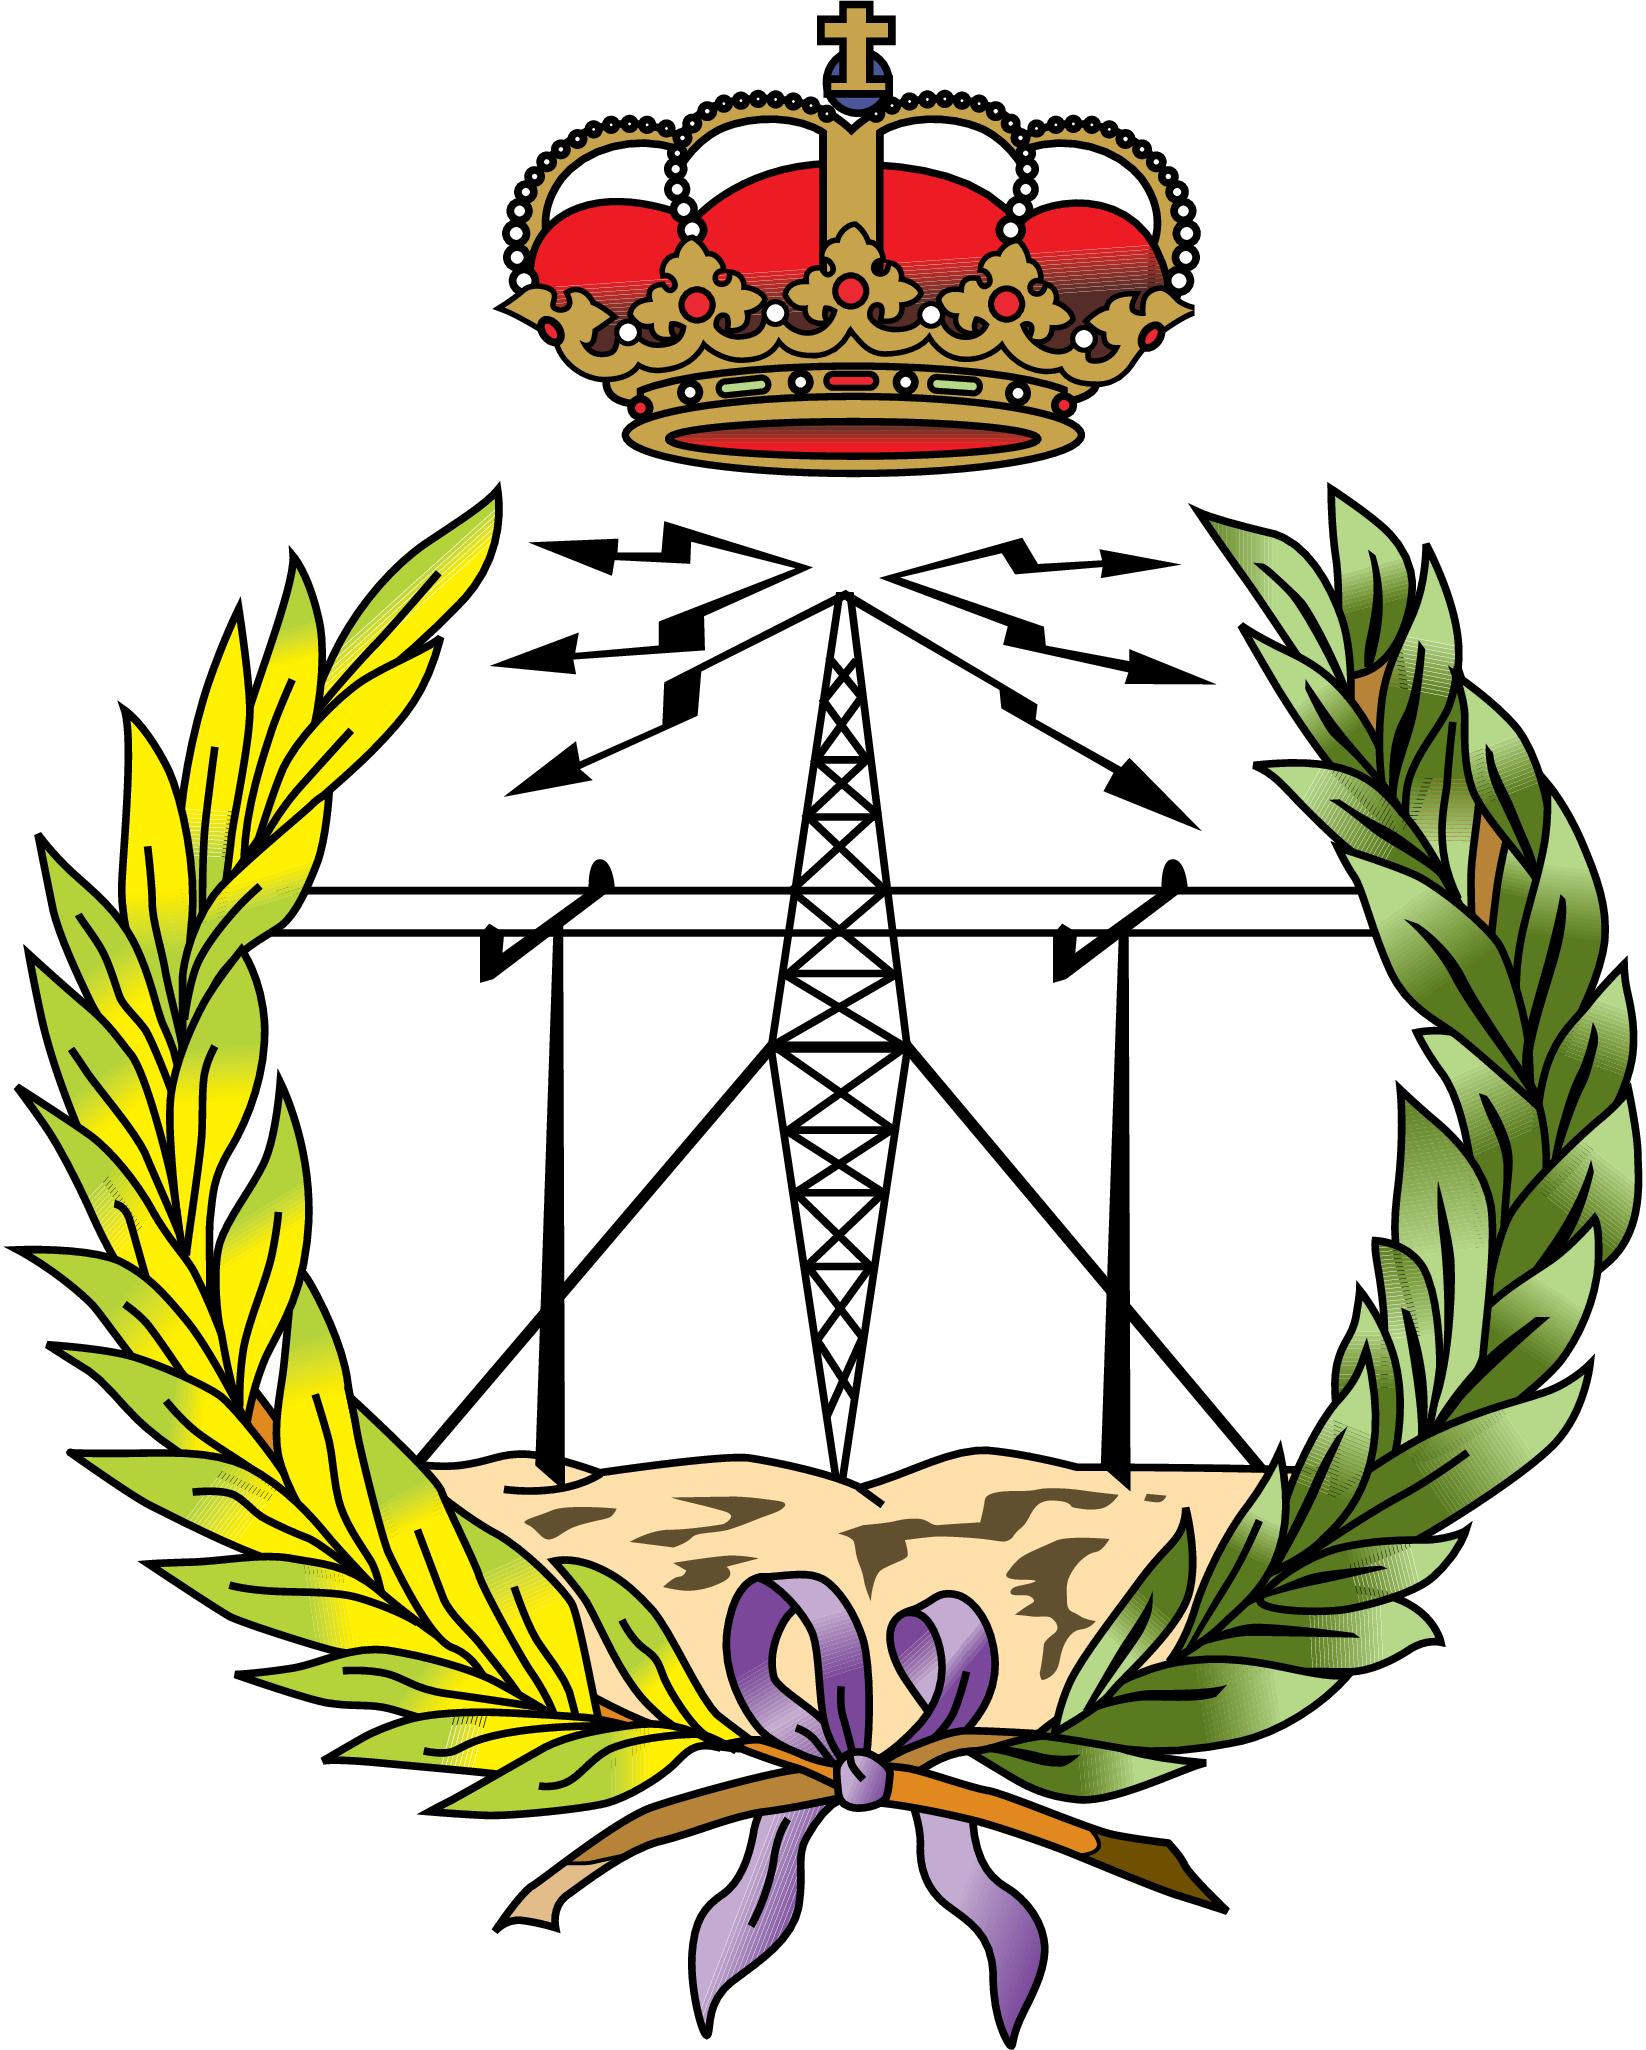
\includegraphics[width=\linewidth]{../../Archivos comunes/etsist_logo.png}
  \end{subfigure}
\end{figure}

% Introducción
\newpage
\phantomsection
\addcontentsline{toc}{section}{Prólogo}
\section*{Prólogo}
Imagen de la portada: \textsl{Título}, por Richard Jhonson.
\newpage

% Índice (TOC)
\setlength{\parskip}{0em}
\tableofcontents
\setlength{\parskip}{0.5em}

%%% INICIO DE LOS APUNTES %%%
\chapter{Introducción a las Redes de Telecomunicación}

\section{Redes y Servicios de Telecomunicación}
\subsection{Red de telecomunicación}
Una red de telecomunicación es un conjunto organizado de \textbf{recursos e información compartidos} por usuarios, que permite el intercambio de información entre entidades distantes.

Estos recursos son un conjunto de \textbf{elementos hardware y software} que ofrecen a la sociedad las \textbf{capacidades de comunicació}n para mejorar la calidad de vida y su desarrollo.

\subsubsection{Características de las redes de telecomunicación}
Una red de telecomunicación tiene varias características:
\begin{itemize}
  \item Se realiza una comunicación entre los miembros de la red, a los que se denomina \textbf{usuarios}.
  \item Una red de telecomunicación permite \textbf{optimizar los recursos} y \textbf{aprovechar las infraestructuras}.
  \item Son \textbf{flexibles} y \textbf{escalables}.
  \item Están \textbf{reguladas} por leyes.
  \item Requieren de un \textbf{mantenimiento} para garantizar el correcto funcionamiento a lo largo del tiempo.
  \item Presentan una \textbf{alta fiabilidad} y son \textbf{interoperables}.
\end{itemize}

\subsection{Componentes esenciales de una red de telecomunicación}
Una red de telecomunicación en realidad es un conjunto de \textbf{nodos} y \textbf{enlaces} que proporciona conexiones entre dos o más puntos de terminación de la red (\textbf{PTR}, por sus siglas). Esta definición excluye los terminales de usuario.

Una red de telecomunicación se puede dividir en:
\begin{itemize}
  \item Sistemas de Transmisión.
  \item Sistemas de Señalización.
  \item Sistemas de Conmutación.
\end{itemize}

\subsection{Servicios de una red de telecomunicación}
Una red de telecomunicación ofrece un conjunto de prestaciones, que reciben el nombre de \textbf{servicios}, y que \textbf{satisfacen las necesidades de comunicación de los usuarios} a través del uso de la red.

Los usuarios no tienen por qué conocer el funcionamiento interno de las redes de telecomunicación. Además, la calidad de estos servicios dependerá de la tecnología empleada en la red.

\subsubsection{Redes y servicios telemáticos}
La \textbf{telemática} engloba la mejora de los actuales mecanismos de telecomunicación y la creación de otros nuevos mediante el uso de sistemas computacionales.

Por lo tanto, las \textbf{redes telemáticas} son redes de telecomunicación basadas en \textbf{sistemas de computación}.

\subsection{Protocolos}
Un \textbf{protocolo} es un \textbf{conjunto de reglas} que determinan el comportamiento de una comunicación. Los protocolos definen el \textbf{formato}, el \textbf{orden} de los mensajes enviados y recibidos entre las entidades de la red y las \textbf{acciones} tomadas al transmitir o recibir mensajes.

Por ejemplo, protocolos pueden ser:
\begin{multicols}{3}
  \begin{itemize}
    \item \textbf{Protocolo humano:}

          \circledNumber{1} --- ¡Hola!

          \circledNumber{2} --- Hola, ¿qué tal?

          \circledNumber{1} --- Bien, ¿y tú?
  \end{itemize}
  \columnbreak
  \begin{itemize}
    \item \textbf{P. de redes de ordenadores:}
          \begin{verbatim}
1. Requerimiento de conexión TCP.
2. Respuesta de conexión TCP.
1. Get "http://www.opm.cl/agv".
2. Envío de archivo.
\end{verbatim}
  \end{itemize}
  \columnbreak
\end{multicols}

\subsection{Redes de acceso}
Una red de acceso es una red que comunica los \textbf{PTR} (puntos de acceso a red) con algún nodo local (el cual forma parte de una red de agregación). Puede haber miles de entidades conectadas a una de estas redes.

\subsection{Medios de transmisión}
Tiene que existir un \textbf{medio físico} para conectar de alguna forma al emisor y al receptor. La transmisión se puede realizar mediante \textbf{ondas electromagnéticas} a través de cables o usando la atmósfera como medio.

Entonces, los medios de transmisión pueden ser:
\begin{itemize}
  \item Metálicos y ópticos (guiados).
  \item Atmósfera (inalámbricos, no guiados).
\end{itemize}

\subsubsection{Metálicos y ópticos}
\vspace{1.5\parskip}
\begin{itemize}
  \item \textbf{Par trenzado.} Un solo cable agrupa 2 o más canales.
  \item \textbf{Cable coaxial.} Un conductor interno de cobre se recubre con un aislante dieléctrico, un blindaje de aluminio, una malla trenzada de cobre/aluminio y una cubierta plástica de PVC.
  \item \textbf{Fibra óptica.} Un núcleo que agrupa varios canales, con revestimiento y protección. Se diferencian de los anteriores porque las señales que se transmiten por estos son ópticas (luz), mientras que en los otros se transmiten señales eléctricas.
\end{itemize}

\subsubsection{Atmósfera}
Cada servicio tiene asignadas unas \textbf{bandas de frecuencia} determinadas. Esto se hace para evitar las posibles interferencias entre señales de servicios diferentes.


\section{Clasificación de las Redes de Telecomunicación}
\subsection{Arquitecturas de red}
Las redes de telecomunicación pueden ser clasificadas según diferentes criterios.
\subsubsection{Clasifiación según el ámbito de las redes}
\vspace{\parskip}
\begin{enumerate}
  \item Redes de área corporal (\textbf{BAN}).
  \item Redes de área personal (\textbf{PAN}).
  \item Redes de área local (\textbf{LAN}).
  \item Redes de área metropolitana (\textbf{MAN}).
  \item Redes de área extensa (\textbf{WAN}). Estas suelen utilizar medios telefónicos. Los servicios son contratados a operadoras (Telefónica, Ono, ...) y suponen un \textbf{coste elevado} de la comunicación. Los enlaces punto a punto pueden ser temporales o permanentes, excepto las comunicaciones vía satélite que son \textsl{broadcast}.

        Hay servicios WAN que son redes de conmutación de paquetes.
\end{enumerate}

\begin{table}[h] \caption{Clasificación de redes por su ámbito}
  \centering
  \begin{tabular}{ | >{\centering}m{14em} | >{\centering}m{11em} | c | }
    \hline
    \textbf{Distancia entre terminales conectados a la red} & \textbf{Terminales ubicados en el mismo...} & \textbf{Posible red} \\ \hline\hline
    En el ámbito del cuerpo humano                          & Cuerpo humano                               & BAN                  \\ \hline
    30 m                                                    & Habitación                                  & PAN                  \\ \hline
    100 m                                                   & Edificio                                    & LAN                  \\ \hline
    1 km                                                    & Campus                                      & LAN                  \\ \hline
    10 km                                                   & Ciudad                                      & MAN (o WAN)          \\ \hline
    100 km                                                  & País                                        & WAN                  \\ \hline
    1.000 km                                                & Continente                                  & WAN                  \\ \hline
    10.000 km                                               & Planeta                                     & WAN                  \\ \hline
  \end{tabular}
\end{table}

\subsubsection{Clasificación según la arquitectura de red y tecnología de transmisión}
\vspace{1.5\parskip}
\begin{itemize}
  \item Redes conmutadas:
        \begin{itemize}
          \item Conmutación de circuitos (por ejemplo, la antigua red telefónica).
          \item Conmutación de paquetes (por ejemplo, Internet).
        \end{itemize}
  \item Redes de difusión.
        \begin{itemize}
          \item Redes de área local.
          \item Redes por radio.
          \item Redes por satélite.
        \end{itemize}
\end{itemize}

\subsubsection{Redes conmutadas}
Las redes conmutadas presentan varios elementos:
\begin{itemize}
  \item \textbf{Nodos de conmutación.} En función del destino, se escoge la ruta y el enlace hacia el nodo siguiente, estableciendo una conexión interna entre el punto de entrada del nodo y otro punto del nodo (salida).
  \item \textbf{Enlaces.} Permiten el transporte de la información (\textbf{señales}) entre nodos, mediante:
        \begin{itemize}
          \item Sistemas de transmisión y radio.
          \item Directamente por medios de transmisión.
        \end{itemize}
  \item \textbf{Red de acceso.} Conecta nodos de acceso y puntos de terminación de red (PTR).
\end{itemize}

\subsubsection{Redes de difusión: radio y televisión}
La señales se difunden a \textbf{múltiples usuarios}. Esto representa una comunicación \textbf{punto-multipunto}.

\subsection{Topologías}
La \textbf{topología} de una red define el modo de interconectar los diferentes elementos de la red. Entre las topologías básicas podemos encontrar:
\begin{multicols}{3}
  \begin{itemize}
    \item Anillo.
    \item Bus.
    \item Estrella.
    \item Malla parcial.
    \item Árbol.
  \end{itemize}
\end{multicols}

Las redes actuales suelen tener una mezcla de topologías. Por ejemplo, una red troncal parcialmente mallada que se combina con una red de acceso en árbol.

\section{Técnicas de conmutación}
\subsection{Conmutación de circuitos}
La conmutación de circuitos es una técnica desarrollada para la \textbf{transmisión de señales vocales}. Un ejemplo es la \textbf{red telefónica conmutada}.

Un \textbf{circuito} es un \textbf{camino dedicado} que se establece entre los terminales de usuario (teléfonos) mientras dura la comunicación.

En este tipo de redes, podemos discernir tres fases:
\begin{enumerate}
  \item \textbf{Establecimiento del circuito} (señalización y encaminamiento).
  \item  \textbf{Transferencia bidireccional de información} (señales vocales).
  \item  \textbf{Liberación del circuito} (señalización y liberación de recursos).
\end{enumerate}

El proceso de elección de rutas y enlaces se realiza solo una vez durante el establecimiento de la comunicación. Además, el \textbf{tiempo de establecimiento} de la comunicación es relativamente \textbf{largo}, aunque se compensa con la baja latencia que experimentan los usuarios una vez se ha establecido la comunicación.

En cuanto al tráfico de voz para usuarios, esta es una técnica que poco a poco va siendo sustituida por la conmutación de paquetes (\textbf{voz sobre IP}, también llamado \textbf{VoIP}). Ahora mismo, los usuarios disponen de fibra óptica en sus domicilios, de modo que se utiliza tecnología digital en la transmisión de voz hasta el proveedor del servicio. Este proveedor conecta entonces con una red de conmutación de paquetes, de modo que pueda operar en VoIP.

\subsection{Conmutación de paquetes}
La conmutación de paquetes es una técnica desarrollada para la \textbf{transmisión de datos}. El mayor ejemplo de este tipo de red es \textbf{Internet}.

La información a transmitir (o mensaje) se divide en unidades más pequeñas denominadas \textbf{paquetes}. Cada paquete tiene una \underline{cabecera}, que corresponde con la gestión interna del mensaje, y \underline{datos de usuario}, que forma parte del propio mensaje.

En los nodos de CP\footnote{CP: onmutación de paquetes.} se realizan, entre otras, las siguientes funciones:
\begin{itemize}
  \item \textbf{Almacenamiento.}
  \item \textbf{Encaminamiento.}
  \item \textbf{Reenvío.}
\end{itemize}

El proceso de elección de rutas y enlaces que se realiza en cada nodo es diferente para cada paquete. Esto quiere decir que, dependiendo de si el funcionamiento interno es de \textbf{datagrama} (NOC)\footnote{NOC: no orientado a la conexión.} o de \textbf{circuito virtual} (OC)\footnote{OC: orientado a la conexión.}, los paquetes no tienen por qué seguir la misma ruta hasta llegar al destino, y pueden no llegar en orden. En tal caso, los paquetes se ordenan cuando ya han llegado al receptor.

El \textbf{enlace entre nodos} se encuentra \textbf{compartido} con otras comunicaciones.

Los terminales y la red pueden controlar la comunicación mediante, por ejemplo, el control de flujo y errores en redes con servicio OC.



\section{Evolución de las redes de telecomunicación}

\subsection{Evolución histórica}
Las primeras redes telefónicas conmutadas surgieron en los años 20 y, como era de esperar, eran analógicas. Por la misma época surgieron también las primeras redes de radiodifusión analógicas. Unos años más tarde, allá por 1937, aparecieron las primeras redes de televisión en blanco y negro.

Después de esto, llegaría la Segunda Guerra Mundial y se produciría una pausa en el desarrollo de las redes de telcomunicación. O, al menos, en parte.

Hacia 1965 surgió la televisión a color y apenas cinco años después aparecieron las primeras redes de conmutación de paquetes. Poco después vinieron las redes telefónicas conmutadas digitales y llegó el \textsl{boom} de Internet, LAN Ethernet, las redes móviles, la World Wide Web...

Por el año 2000 la televisión pasó a formato digital y, poco a poco, se está dando una digitalización de todas las redes. Otro ejemplo son las redes telefónicas analógicas, que estan desapareciendo paulatinamente para dejar paso a VoIP.

\subsection{Internet}
Internet es un conjunto de redes de ámbito mundial que permite la interconexión de millones de dispositivos (sistemas terminales o \textbf{hosts}) y \textbf{redes privadas}, donde se ejecutan las \textbf{aplicaciones distribuidas} (Web, \textsl{e-mail}, juegos, \textsl{e-commerce}, compartición de archivos, etc.).

La infraestructura de las comunicaciones que se realizan en Internet está compuesta por:
\begin{itemize}
  \item Conmutadores de paquetes (\textbf{routers}).
  \item \textbf{Sistemas de transmisión, radio y satélite}.
  \item Un conjunto de \textbf{protocolos} normalizados.
\end{itemize}

\chapter{Arquitecturas de comunicación estratificadas en niveles}


Un \textbf{protocolo} es un conjunto de reglas que determinan el comportamiento de la comunicación entre entidades pares. Siempre se produce entre entidades pares.

En una comunicación vertical, se denominan \textbf{entidades adyacentes} a aquellas entidades que se comunican directamente entre ellas.

Un \textbf{servicio} es la capacidad que tiene un nivel y que se ofrece al nivel superior para que éste la use. El servicio se ofrece y se recibe entre entidades adyacentes.

Una \textbf{interfaz} es la forma de comunicación entre niveles adyacentes. Es un problema local.

Entre entidades pares hay \textbf{protocolos}.




\section{Arquitecturas de comunicación estratificadas en niveles}
\subsection{Conceptos generales}
\subsubsection{¿Por qué es necesaria una arquitectura de protocolos?}
En el intercambio de datos entre ordenadores, los procedimientos pueden llegar a ser bastante complejos. Además, es muy difícil intentar abordar la solución como un todo. Debemos hacer acopio de la frase \textsl{divide y vencerás}.
Lo que pretendemos es ir resolviendo problema a problema, de forma que la solución de cada uno servirá de base para poder obtener la solución del siguiente.

Con la arquitectura de protocolos se procura determinar las funciones a realizar y establecer capas o \textbf{niveles}. Cada nivel tiene asignadas unas funciones o \textbf{servicios} que proporciona a otro nivel, de modo que solo se debe preocupar de sus propios servicios y los demás no tienen por qué conocer su funcionamiento.

Por ejemplo, si hay empresario que quiere enviar un PDF encriptado a otro empresario, le pedirá a un servicio de criptografía que le encripte el archivo para luego poder mandarlo. El servicio de criptografía no tiene por qué saber de economía, ni el empresario de encriptado de PDFs.

\subsubsection{Estratificación en niveles}
Cada nivel usa los servicios del nivel inmediatamente inferior. Es decir, que un nivel solo puede ofrecer servicios al nivel superior.

El nivel que usa los servicios del nivel inmediatamente inferior recibe el nombre de \textbf{usuario}, mientras que aquel nivel que le proporciona los servicios se denomina \textbf{proveedor}.

El nivel inferior no modifica ni interpreta los datos del nivel superior. En otras palabras, los niveles son \textbf{independientes} entre sí, pero no son \textbf{indiferentes}.

\subsubsection{Tipos de comunicación}
En una arquitectura estratificada, se pueden distinguir dos tipos de comunicación:
\begin{enumerate}
  \item \textbf{Comunicación horizontal.} Es la que se consigue entre entidades del mismo nivel. Es una comunicación \textbf{virtual}, ya que no se produce de forma directa entre las entidades (excepto si se trata del último nivel de la arquitectura, el que hace de enlace con el medio físico).
  \item \textbf{Comunicación vertical.} Se produce en entre entidades de dos niveles adyacentes. Representa el \textbf{flujo real} de la información.
\end{enumerate}

Cada nivel debe definir con precisión:
\begin{itemize}
  \item La \textbf{especificación del servicio}, que es la interfaz que se usará con el nivel superior para ofrecer los servicios.
  \item La \textbf{especificación de protocolo}, que describirá la sintaxis y la semántica de las PDU\footnote{PDU: \textsl{Protocol Data Unit}.}.
\end{itemize}

\begin{multicols}{2}
  \subsubsection{Comunicación horizontal}
  Las entidades de un mismo nivel que se comunican entre sí se denominan \textbf{entidades pares} y tendrán igual comportamiento y jerarquía.

  Las entidades pares se comunican horizontalmente mediante \textbf{protocolos de pares}. Estos, como cualquier otro protocolo, son un conjunto de reglas que determinan el comportamiento de la comunicación entre entidades pares.
  \columnbreak
  \subsubsection{Comunicación vertical}
  Las entidades en una misma torre de comunicaciones que se comunican entre sí se denominan \textbf{entidades adyacentes}.

  Un \textbf{servicio} es un conjunto de facilidades que un nivel (\textbf{proveedor}) ofrece al nivel inmediatamente superior (\textbf{usuario}), para que este las use.

  Una \textbf{interfaz} es la ``frontera'' entre dos niveles. \textbf{Definir una interfaz} significa establecer la forma de comunicación entre dos niveles adyacentes. Es un problema exclusivamente \textbf{local}.

  Un nivel $N$ ofrece un servicio al nivel superior $(N+1)$ pero es usuario del nivel inferior $(N-1)$.

  Un nivel usa los servicios del nivel inferior accesibles a través de los \textbf{\textsl{Service Acess Point} (SAP)}. Cada SAP representa el punto en que se puede obtener un servicio determinado.
\end{multicols}

\subsection{Conceptos: entidad, unidad de datos, protocolo}
\subsubsection{Especificacion de un protocolo}
\vspace{1.5\parskip}
\begin{itemize}
  \item Se debe definir el \textbf{formato} que tendrán las PDU. Estas tendrán dos partes bien diferenciadas:
        \begin{itemize}
          \item Los \textbf{datos} del nivel superior conformarán la SDU\footnote{SDU: \textsl{Service Data Unit}.}.
          \item Los parámetros de \textbf{control} formarán la PCI\footnote{PCI: \textsl{Protocol Control Information}.}. Estos parámetros de control necesarios para que dos entidades de nivel $N$ puedan cooperar en la provisión de un servicio
        \end{itemize}
  \item Definición de las \textbf{acciones y respuestas} al transmitir (o recibir) las distintas PDU.
\end{itemize}

\subsubsection{Encapsulado de PDUs}
Para que se llegue a producir la comunicación horizontal, se tendrá que realizar una comunicación vertical entre los niveles $(N)$ y $(N-1)$, posteriormente entre los niveles $(N-1)$ y $(N-2)$, y así hasta llegar al nivel de enlace con el medio físico. Después, se realizará de nuevo la comunicación vertical, pero en la torre de la entidad par y en sentido ascendente.

Imaginemos que del nivel $(N+1)$ llega una PDU que llamaremos $(N+1)$PDU. Esta será la SDU del nivel $N$. Luego, se le añade una información de control, es decir, una $(N)$PCI. Lo puedes ver mejor en la \autoref{fig:encapsulado_de_PDU}.

\begin{figure}[ht]
  \centering
  \begin{tikzpicture}[auto,>=latex']
    \node [input, name=input] (input) {};
    \node [block, below of=input, node distance=0cm] (nmasuno) {$(N+1)\text{PDU}$};

    \node [block, below of=nmasuno, node distance=2cm] (bloquensdu) {$(N)\text{SDU}$};
    \node [block, left of=bloquensdu, node distance=1.6cm] (bloquenpci) {$(N)\text{PCI}$};
    \node [draw, inner sep=8pt, fit=(bloquensdu) (bloquenpci)] (bloquen) {};
    \node [text width=120pt, align=center, below of=bloquen, node distance=1.1cm] (text1) {$\underbrace{\phantom{(N)\text{SDU}\qquad\qquad  (N)\text{PCI}}}_{\displaystyle{(N)\text{PDU}}}$};

    \node [block, below of=text1, node distance=2.2cm] (bloquenmenos1sdu) {$(N-1)\text{SDU}$};
    \node [block, left of=bloquenmenos1sdu, node distance=2.2cm] (bloquenmenos1pci) {$(N-1)\text{PCI}$};
    \node [draw, inner sep=8pt, fit=(bloquenmenos1sdu) (bloquenmenos1pci)] (bloquenmenos1) {};
    \node [text width=150pt, align=center, below of=bloquenmenos1, node distance=1.1cm] (text2) {$\underbrace{\phantom{(N-1)\text{SDU}\qquad\qquad  (N-1)\text{PCI}}}_{\displaystyle{(N-1)\text{PDU}}}$};

    \node [text width=3cm, right of=nmasuno, node distance=3.2cm] (text3) {$\sim N+1$};
    \node [text width=3cm, below of=text3, node distance=2cm] (text4) {$\sim N$};
    \node [text width=3cm, below of=text4, node distance=3.3cm] (text5) {$\sim N-1$};

    \node [text width=3.2cm, left of=bloquenpci, node distance=3.5cm] (text6) {Metemos la información de control.};
    \node [text width=3.2cm, left of=bloquenmenos1pci, node distance=3.5cm] (text7) {Metemos la información de control.};

    \draw [-angle 90] (nmasuno) --  node{} (bloquensdu);
    \draw [-angle 90] (text1) --  node{} (bloquenmenos1sdu);
    \draw [-angle 90] (text6) --  node{} (bloquenpci);
    \draw [-angle 90] (text7) --  node{} (bloquenmenos1pci);
  \end{tikzpicture}
  \caption{Encapsulado de PDUs} \label{fig:encapsulado_de_PDU}
\end{figure}

\subsubsection{Tipos de PDU}
Existen dos tipos diferentes de PDU:
\begin{enumerate}
  \item \textbf{PDU de datos.}Llevan información de interés para la entidad par (información de control) y transportan de manera transparente la información del nivel superior (datos).
  \item \textbf{PDU de control.} Llevan información de interés únicamente para la entidad par (información de control). Si te fijas de nuevo en la \autoref{fig:encapsulado_de_PDU}, concretamente en el nivel $N$, sería como si la parte de $(N)$SDU estuviera vacía, solo contendría la $(N)$PCI.
\end{enumerate}

\subsection{Modelos de referencia}

Los modelos de referencia\footnote{Un modelo es una simplificación de la realidad. Proporciona los ``planos de un sistema''. Los modelos se construyen para comprender mejor el sistema que se está desarrollando.} definen el \textbf{proceso global de las comunicaciones}. Por tanto, sirven de referencia en el diseño de redes y aplicaciones. Estos modelos también definen \textbf{procesos normalizados} para la interconexión de sistemas y el intercambio de información entre usuarios. Además, realizan una \textbf{aproximación por niveles}, agrupando funcionalidades similares en un mismo nivel y describiendo el comportamiento de cada nivel (pero no su implementación).

El uso de los modelos de referencia conlleva unas ciertas ventajas:
\begin{itemize}
  \item Independencia de los dispositivos y fabricantes.
  \item Facilidad de adaptación a los cambios tecnológicos.
  \item Mayor disponibilidad y eficiencia del sistema.
\end{itemize}

Para más información sobre los modelos de referencia, ver la \autoref{sec:modelos_de_referencia}.

\subsection{Ejemplo: Cliente - Servidor WEB}
En esta situación, el proceso cliente realiza peticiones de páginas web y los servidores web proporcionan las respuestas.

El protocolo que se usa es \textbf{HTTP}\footnote{HTTP: \textsl{Hyper Text Transfer Protocol}.}, el cual especifica cómo interacciona el cliente y el servidor web (las entidades de comunicación).

\begin{figure}[ht!]
  \centering
  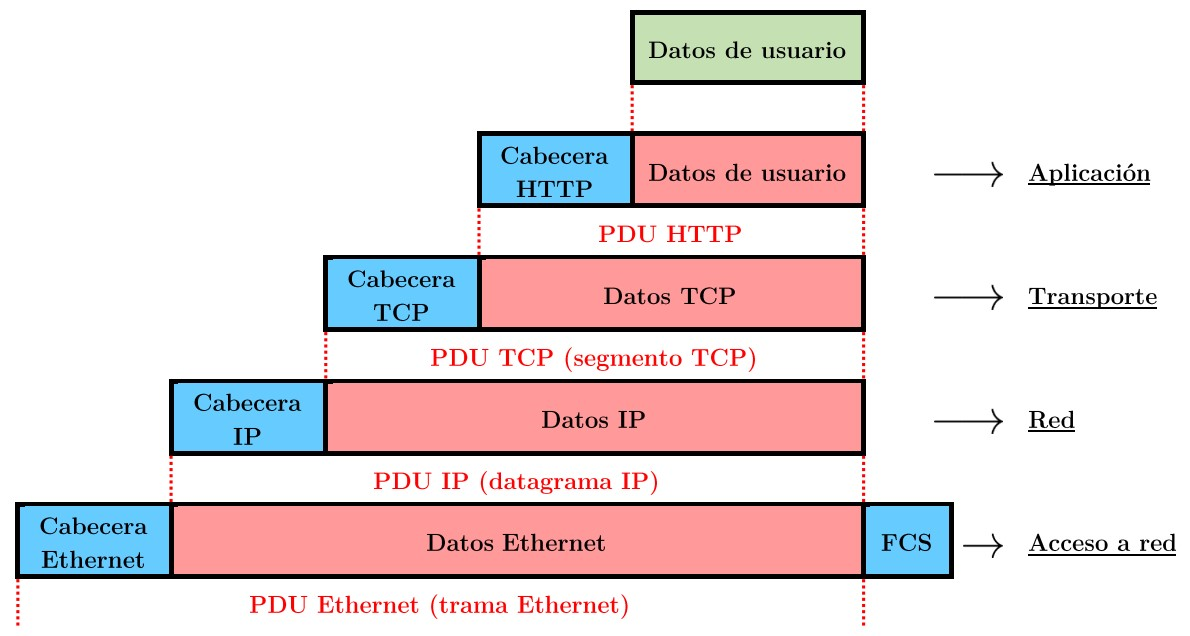
\includegraphics[width=\linewidth]{./Imágenes/aaa.jpg}
  \caption{Encapsulado de PDU de una comunicación cliente - servidor WEB.}
\end{figure}


\newpage
\section{Interacción entre entidades y niveles}
\subsection{Tipos de primitivas y clases de servicio}
Un servicio se solicita y se obtiene por medio de un conjunto de operaciones o funciones denominadas \textbf{primitivas}.

Existen varios tipos de primitivas:
\begin{multicols}{2}
  \begin{enumerate}
    \item \textsl{Request}
    \item \textsl{Response}
    \item \textsl{Indication}
    \item \textsl{Confirm}
  \end{enumerate}

\end{multicols}
Una primitiva se implementa en un lenguaje de programación como una \textbf{función} o \textbf{método} (con un conjunto de parámetros) que realiza una operación. Un ejemplo de uso de primitivas en Java sería:

\begin{lstlisting}
envia(datos,long,org,dst);
socket.send(datagrama);
\end{lstlisting}

Existen distintas clases de servicio, dependiendo del tipo de primitivas que hayan definido para el mismo.
\begin{itemize}
  \item \textbf{Servicio confirmado por el usuario remoto.} \begin{verbatim}
Request --> Indication --> Response --> Confirm
\end{verbatim}
  \item \textbf{Servicio no confirmado.}
        \begin{verbatim}
Request --> Indication
\end{verbatim}
  \item \textbf{Servicio confirmado por proveedor local.}
        \begin{verbatim}
         --> Indication
Request
         --> Confirm
\end{verbatim}
  \item \textbf{Proveedor del servicio notifica de un evento.}
        \begin{verbatim}
Indication
\end{verbatim}
\end{itemize}


\subsection{Modelo Internet}
\subsubsection{Puertos}
Los \textbf{puertos} se utilizan en el nivel de transporte para direccionar las distintas aplicaciones (procesos). Un puerto no es nada más que el \textbf{identificador del SAP del nivel de transporte}.

Cada máquina disponde de 65535 puertos.

El rango de puertos (1 ... 1023) se denominan \textbf{puertos reservados} o \textbf{\textsl{well-known}} y se utilizan en la parte servidora de los procesos para proporcionar los servicios de red más comunes:
\setlength{\columnsep}{-5cm}
\begin{multicols}{2}
  \begin{itemize}
    \item Puerto 7: \verb!echo!
    \item Puerto 13: \verb!daytime!
    \item Puertos 20 y 21: \verb!FTP! (transferencia de ficheros)
    \item Puerto 80: \verb!web-http!
  \end{itemize}
\end{multicols}

Los puertos \textbf{a partir de 1024} son \textbf{puertos no reservados}, se utilizan en la parte cliente de los procesos para acceder a los servicios de red.

\subsubsection{Socket}
Para facilitar a los programadores de aplicaciones la comunicación entre procesos cliente-servidor, se ha definido una interfaz normalizada denominada \textbf{interfaz de Socket}. Esta interfaz proporciona los métodos o funciones para que los procesos puedan comunicarse.

Un punto extremo (\textbf{socket}) identifica la tupla formada por \textbf{(dirección IP, puerto)}. De esta forma, el proceso queda perfectamente identificado.

Por ejemplo: \verb!(142.0.1.24, 1880)!


\section{Modos de comunicación entre entidades pares}
Existen dos modos principales de comunicación entre entidades pares:
\begin{enumerate}
  \item \textbf{Orientado a la conexión} (\textsl{connected-oriented})

        Se produce un intercambio de datos entre entidades pares a través de una conexión establecida previamente por el nivel inferior. Además, se garantiza la entrega y el orden de llegada de los datos.
  \item \textbf{No orientado a la conexión} (\textsl{connectionless})

        Se produce un intercambio de datos entre entidades partes sin establecimiento previo de una conexión por el nivel inferior. Además, no se garantiza la entrega ni el orden de llegada de los datos.
\end{enumerate}

\section{Conexiones y envío de datos sin conexión}

\subsection{Conexiones}
Una \textbf{conexión} $\mathbf{N}$ es una asociación establecida por el nivel $N$ (\textbf{servicio ofrecido por el nivel} $\mathbf{N}$) para la transferencia de datos entre \textbf{dos entidades} $\mathbf{N+1}$.

Para establecer una conexión $N$, la entidad $N+1$ debe conocer la dirección del $(N)$SAP origen y del $(N)$SAP destino.

La conexión es un servicio confirmado por el usuario remoto y tiene tres fases:
\begin{enumerate}
  \item Establecimiento de la conexión.
  \item Transferencia de datos.
  \item Liberación de la conexión.
\end{enumerate}

El establecimiento de una conexión $N$ entre entidades pares requiere que se lo permitan las entidades pares del nivel inferior $N-1$.

El nivel $N$ puede ofrecer el servicio de conexión aunque el nivel $N-1$ no lo ofrezca.


\subsection{Envío de datos sin conexión}
En el caso de intentar un envío de datos en el nivel $N+1$ sin que exista una conexión establecida, se debe incluir la \textbf{dirección de destino} en la $(N)$PCI.

\section{Facilidades adicionales ofrecidas por un nivel}
\subsection{Control de flujo}
\subsection{Control de errores}

\section{Normalización en redes}
En los orígenes de las redes de telecomunicación no existía la normalización. Esto conducía a una proliferación desordenada de soluciones que resultaban incompatibles entre sí. Además, algunas otras consecuencias eran la baja conectividad, el elevado coste para el usuario e innumerables interfaces de comunicación que dependían del fabricante.

El \textbf{objetivo} de la normalización en las redes, al igual que en cualquier otro ámbito, es facilitar el intercambio de información entre sistemas (elementos) de distintos fabricante, arquitectura o sistema operativo.

Las ventajas principales que ofrece la normalización de las redes son:
\begin{itemize}
  \item Interoperabilidad y/o interconectividad.
  \item Nuevos mercados e incremento de la competencia.
  \item Tendencia a la innovación y a la reducción de costes.
\end{itemize}

Sin embargo, la normalización de las redes también puede traer consigo algunos inconvenientes. Entre ellos:
\begin{itemize}
  \item Ralentización de las soluciones tecnológicas.
  \item Existencia de múltiples estándares para las mismas funciones.
\end{itemize}
\section{Modelos de referencia} \label{sec:modelos_de_referencia}





\chapter{Introducción a los protocolos y servicios de seguridad}


\section{La problemática de la seguridad en las redes}

\section{Servicios de seguridad}

\section{Criptografía de clave secreta y clave pública}

\section{Firma digital}

\section{Certificación digital}




\chapter{Arquitectura de los centros de conmutación y señalización en redes de telecomunicación}


\section{Redes de conmutación de circuitos}

\section{Redes de conmutación de paquetes}

\section{Ejemplificación Redes IP}





\chapter{Prácticas}

\section{Generación y análisis de tráfico de voz sobre IP (VoIP)}

\section{Análisis de protocolos. WireShark}

\section{ Análisis y Diseño de un protocolo de comunicación (NOC y OC)}

\section{Uso de un certificado de clave pública}

%%% FIN DE LOS APUNTES %%%

%%% BIBLIOGRAFÍA %%%
% Por defecto, se encuentra desactivada. Esto disminuye el tiempo de procesado. Se puede activar cuando se vaya a exportar el PDF definitivo

%\newpage
%\phantomsection
%\label{sec:bibliografia_final}
%\renewcommand{\refname}{Bibliografía}
%\addcontentsline{toc}{section}{Bibliografía}
%\bibliography{bibliografia} % Nombre del archivo (sin ".bib")
%\bibliographystyle{bababbrv} 

\end{document}
